
\chapter{Problemy i rozwiązania, testy}

\section{Problemy i rozwiazania}

\section{Testy wydajnościowe i jakościowe}

\begin{center}
	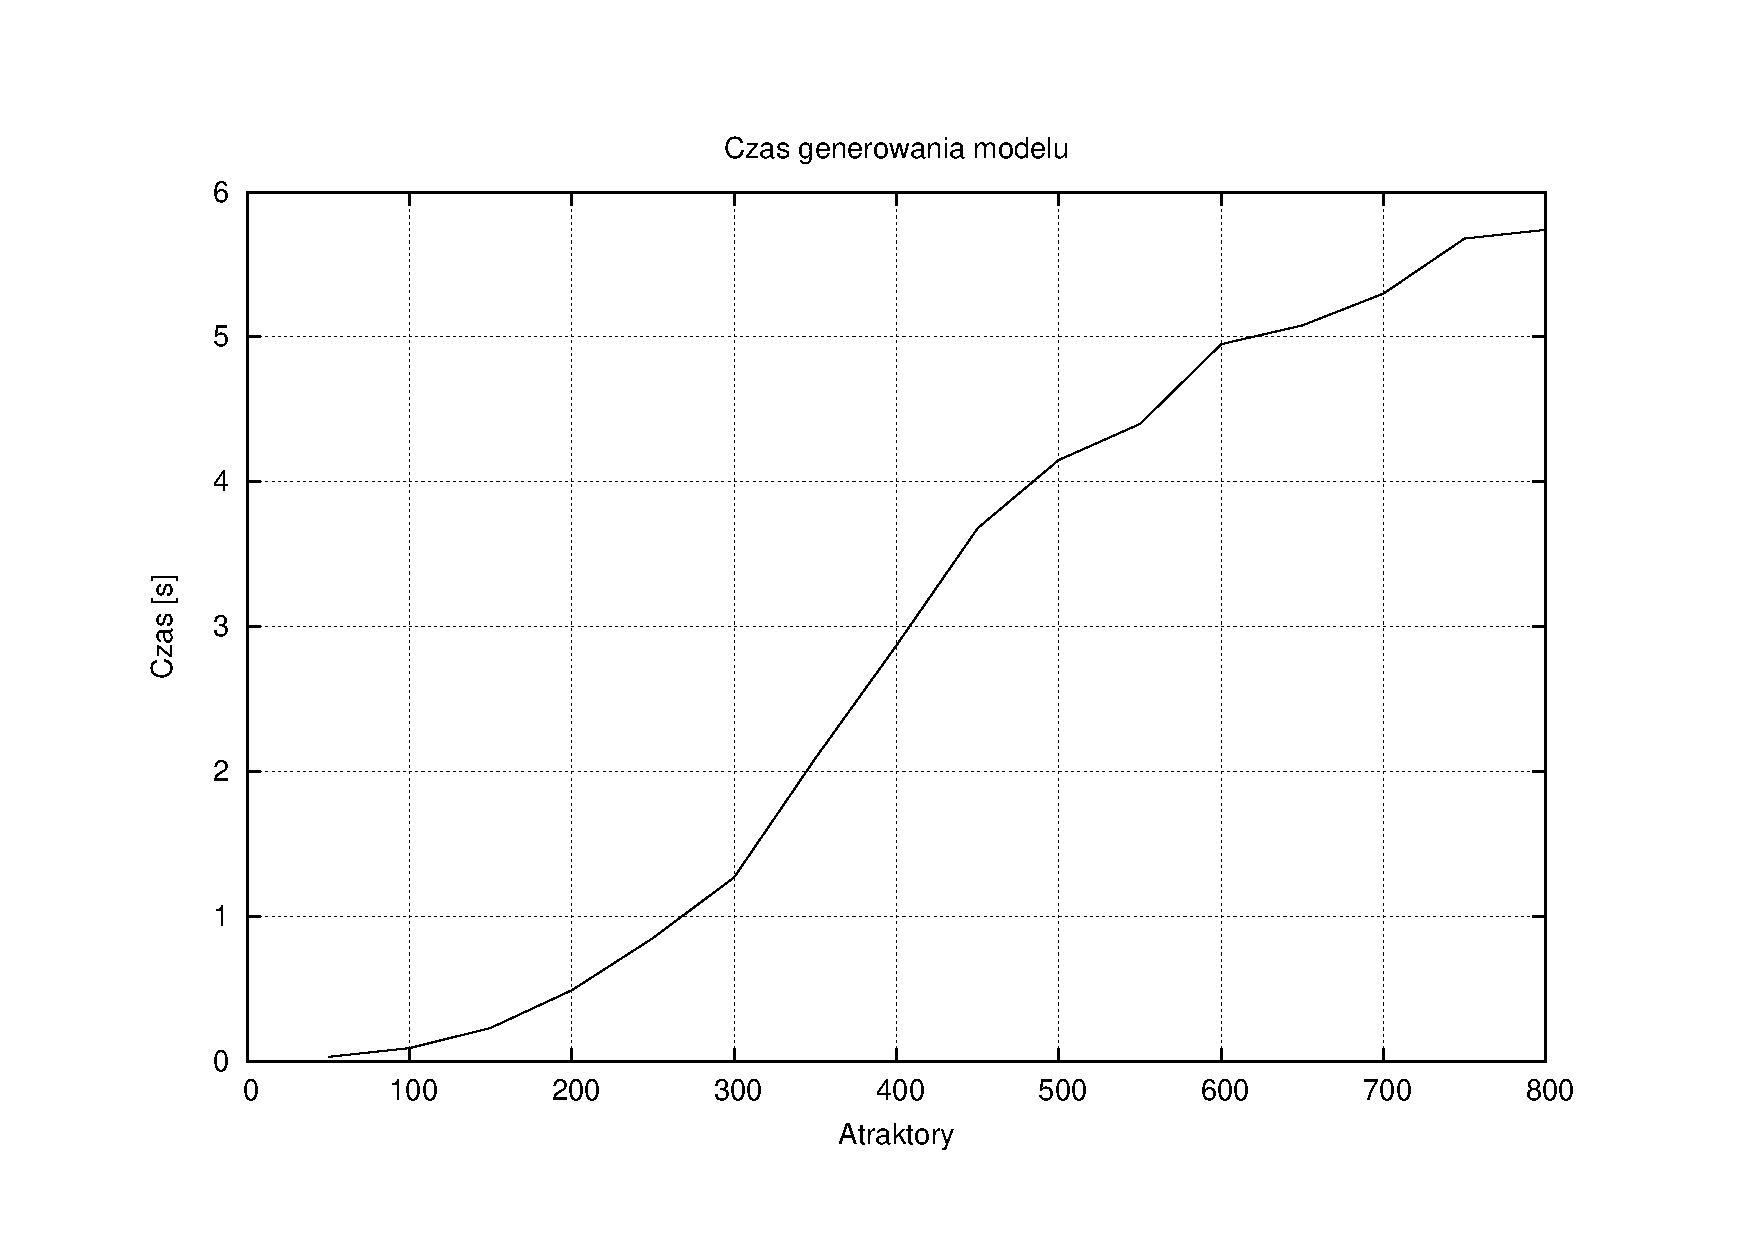
\includegraphics[width=110mm]{images/performance.pdf}
	\captionof{figure}{Czas generowania modelu w zależności od liczby atraktorów.}
\end{center}


\section{Przykladowa galeria z parametrami uzytymi do generowania}

\begin{center}
	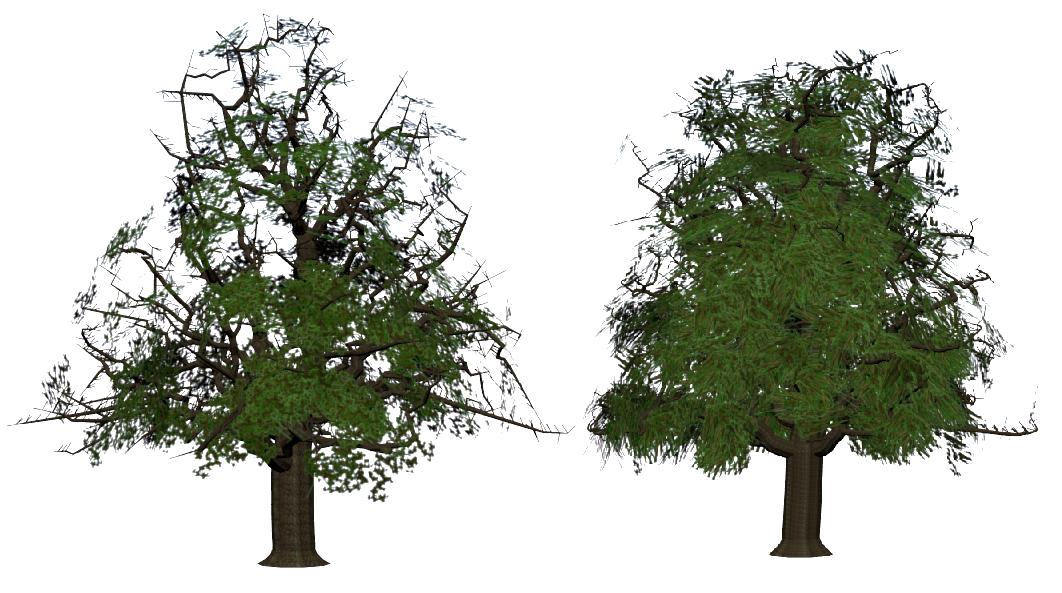
\includegraphics[width=100mm]{images/renders/greentree.png}
	\captionof{figure}{Wpływ liczby liści na wygląd drzewa}
\end{center}

\begin{center}
	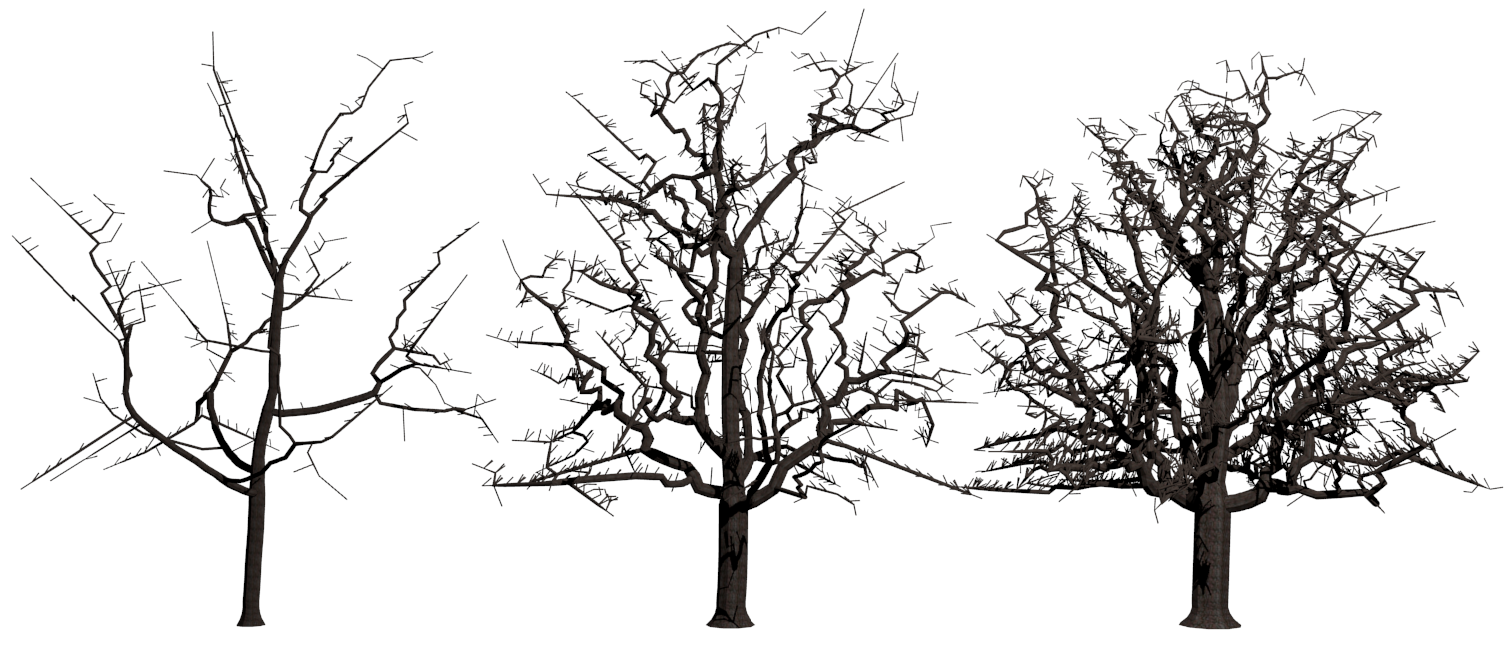
\includegraphics[width=120mm]{images/renders/points.png}
	\captionof{figure}{Wpływ liczby atraktorów na wygląd drzewa}
\end{center}

\begin{center}
	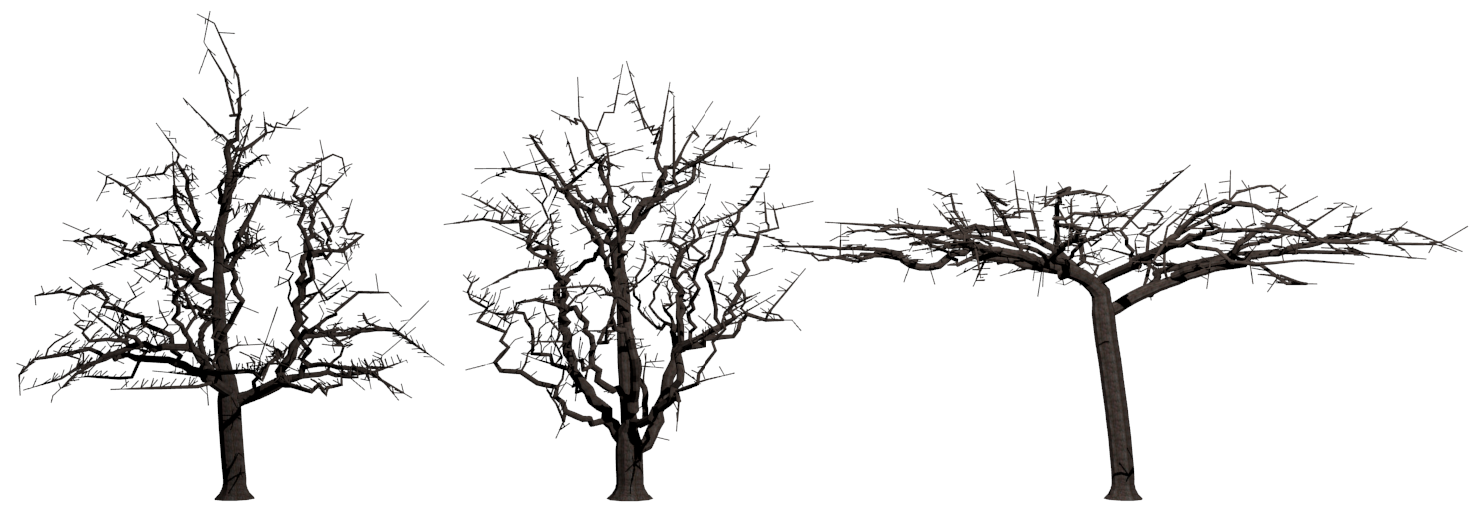
\includegraphics[width=120mm]{images/renders/shape.png}
	\captionof{figure}{Wpływ kształtu korony na wygląd drzewa}
\end{center}

\begin{center}
	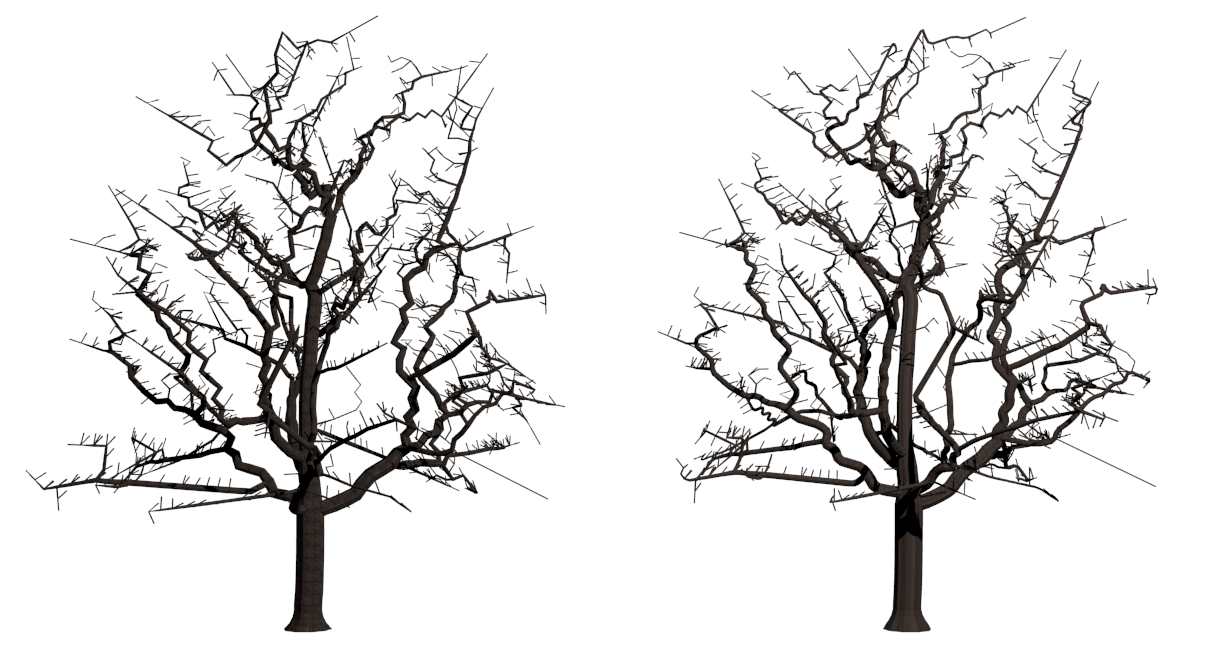
\includegraphics[width=120mm]{images/renders/smooth.png}
	\captionof{figure}{Wpływ wygładzania gałęzi na wygląd drzewa}
\end{center}


